\chapter{Swampland Programs}
\label{Chapter1}
This chapter will be devoted to the introductions of the Swampland programs. In the first section, we will review some basics of the effective field theory. Then, with certain understandings of EFTs, the following sections will introduce concepts of the Swampland, and the Swampland programs. To keep things focused for the purpose of this thesis, stresses are mainly put on the Swampland Distance Conjecture. For statements and discussions about other conjectures and relations between them, we will provide useful references.
\section{Effective Field Theory}
Nature around us comes from a lot of factors. From the perspective of physics, physical phenomena occur in a variety of scales of size: from electrons, nuclei, atoms, molecules to planets, stars, glaxies, and so on. Physics have benn progressing because scientists could undertand them independently without necessity of understanding all of them at once. What made it possible is a property of nature called decoupling, which claims that most of information regarding physics at short distance scale has nothing to do with ones at long-distance scale. For instance, suppose a grass of water which consists of numerous $H_{2} O$ molecules. Each molecule is made from atoms which involve electrons executing orbits around a nucleus. A nucleus itself is consisting of protons and neutrons, and there are more complicated structures as we inquire into it deeper and deeper. However, we are accustomed to be able to know the dynamics of water without knowing such complex structure. The notion of decoupling is important because in some case it is not necessary to know about the detailed properties of nuclei in order to unravell the atomic physics, just as ignoracne about atoms does not keep us from understanding of laws of nature at larger scales such as fluid dynamics and motions of springs. Laws of nature are also described by quantum field theories (QFTs), which shares the property of decoupling. When a particular QFT for short-distance physics is investigated, it is apparently useful if we are able to identify which observables are relevant for a description of the theory and those from which they decouple. A mathematical tool for exploiting the property of decouple is effective field theories (EFTs). Since the Swampland program involves EFT coupled to gravity, in this chapter, we will review some basics of EFTs. Useful reference for this section might be as \parencite{burgess_introduction_2020}. 
\subsection{Basic Ideas}
As stated above, the key idea behind EFTs is that physics is symplified when viewed from a distance. For instance, suppose a system of electric charges within a region of a space of characteristic size $\sim l$. If one may want to study their effects at a distance much larger than $l$, $r \gg l$, detailed knowledge of the charge distribution is not required. Instead, one can approximate the system by a few terms in the multipole expansion, such as the total charge, the dipole moment, and so on. This is the same for particle physics. However, it is more common to use the energy scale rather than the length scale $E = l^{-1}$ to distinguish different regimes. Thus, long distances can be interpreted as low energies. In this sense, experiments with the characteristic energy of order $E$ do not require detailed knowledge of physics at higher energy scales $\Lambda \gg E$. The property of decoupling enable us to pursue particular physics by separating theoretically the system with various energy scales when entire theories (full theories) are still unknown. In addition, even if full theories or other EFTs at higher energy scales are known, EFTs are great tools to symplify their computations by lowering scales.  



\section{The Swampland Program}
In the previous section, the concepts of EFTs were reviewed. Thanks to the property of the decoupling, we are able to study physics starting from low-energy regimes where we are supposed to have enough knowledge without knowing anything about high-energy scale physics. This also enables us to scrutinize physics in higher energy scales beginning from a low energy EFTs whose structures are well-understood. However, how far is this procedure valid? In other words, is there a specific energy scale above which this "bottom-up" study ceases to work? Let us think about the black hole and the Schwarzschild radius $R_{s}$. As the mass increases (i.e. the energy increases), and finally becomes Planck scale $M \sim m_{p} \sim 10^{28} \text{eV}$, the Compton wavelength is shorter than the Schwarzschild radius, and therefore the more detailed structures are hiding behind the event horizon. In this sense, Planck scale might be where the structure of EFTs will be collapsing. In addition, in order to describe physics at Planck scale, it is believed that the theory of qunatum gravity is needed. Hence, if we take quantum gravity into acccount, not all low-energy (IR) EFTs which seem to be consistent are valid at Planck scale. That is, there are supposed to be subsets of EFTs that are inconsistent in consideration of quantum gravity inside the entire set of consistent effective QFTs. This is the emergence of the idea of the Swampland, and necessity of the Swampland program. The aim is, roughly speaking, to determine conditions which distinguish such subsets. In this section, we will introduce the concept of the Swampland, and provide few conjectures needed for the purpose of this thesis. Possible references for this section are \parencite{agmon_lectures_2022}. 

\subsection{The Swampland and The Swampland Program}
From the EFTs perspective, at an energy scale much smaller than Planck scale, we can exploit the decoupling property to study low-energy physics. And once a theory below a certain energy is well understood, we proceed to investigate a new physics whose scale is a little higher than former one's. By repeating this process, EFTs have been thought of as approaches to unknown ultraviolet physics. Nevertheless, at Planck scale, where it is believed that quantum gravity has to be taken into account, it is predicted that the structure of EFTs will be problematic. Normally, when phenomenological problems are considered, since the energy scale is typically much smaller than Planck scale, the effect of the gravity can be ignored or considered classically. While in the case when the energy scale is extremely high, we have to think about the quantization of gravity, it has been believed as an independent problem at a UV scale. Recent researches, however, have been revealing the possibilities that requirements of consistency by quantum gravity are expected to have certain restrictions on its infrared (IR) low-energy physics. This observation suggests that, on the contrary to the EFTs property of decoupling, low-energy phenomenological problems and UV quantum gravity are closely related to each other, and should not be considered independently.
\begin{figure}
    \centering
    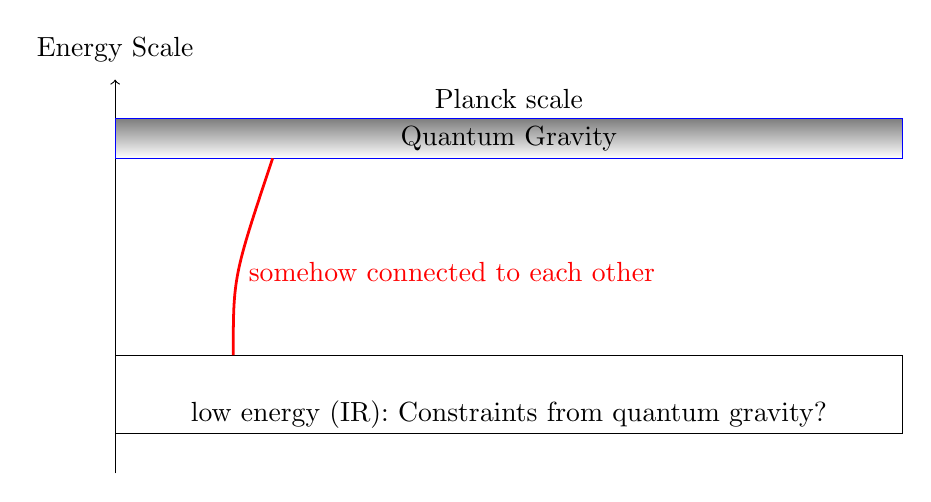
\begin{tikzpicture}[scale=5]
        \draw[->] (0,0) -- (0,1) node[above=3pt]{Energy Scale} ;
        \shadedraw[blue] (0, 0.8) rectangle (2, 0.9);
        \draw (0, 0.1) rectangle (2, 0.3);
        \draw (1,0.85) node{Quantum Gravity};
        \draw (1, 0.95) node{Planck scale};
        \draw (1, 0.15) node{low energy (IR): Constraints from quantum gravity?};
        \draw[line width=1pt, red] (0.3,0.3) .. controls(0.3, 0.5) .. (0.4, 0.8) node[pos = 0.5, right]{somehow connected to each other};
    \end{tikzpicture}
    \caption{On the contrary to the EFTs feature of UV/IR decoupling, it is suggested that low-energy physics is not independent of extremely high-energy theories (quantum gravity).}
    \label{fig:UV/IR mixing}
\end{figure}
Below Planck scale, $M_{p}$, theories can be described by an EFT coupled to classical gravity, since effect of quantum gravity is ignored. Picking a theory of quantum gravity, we can find one low-energy EFT corresponding to such theory at Planck scale. Now let us consider oppositely. That is, if we consider an EFT, can we obtain a theory of quantum gravity which is compatible with it? The answer to this question separates the entire set of EFTs coupled to gravity into two subsets. One is the set of EFTs obtained as consistent low-energy theories of quantum gravity, and the other is its complementary which cannot be valid ones. Former is called the landscape, and latter is the Swampland.

\begin{tcolorbox}[title=The Swampland,
    title filled=false,
    colback=blue!5!white,
    colframe=blue!75!black]
    The set of consistent low-energy EFTs that seem to be consistent, but cannot be compatible in consideration of quantum gravity.
\end{tcolorbox} 
\begin{figure}
    \centering
    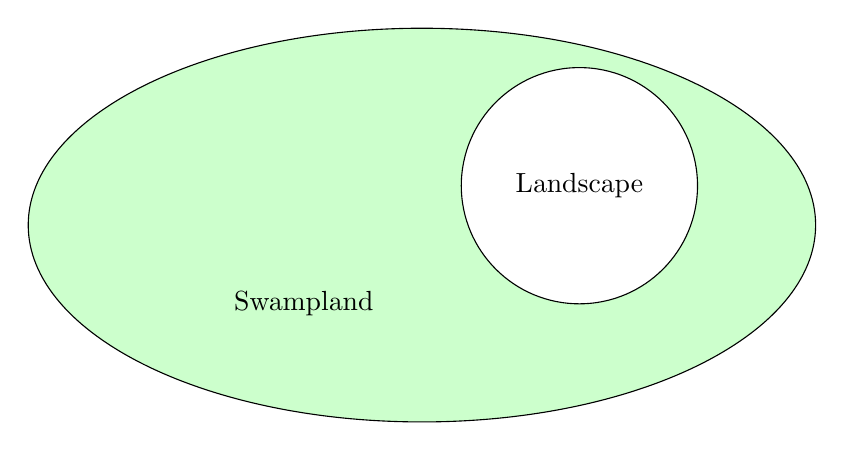
\begin{tikzpicture}[scale=5]
        \draw[fill= green!20] (0,0) ellipse (1 and .5);
        \draw[fill=white] (0.4,0.1) circle (.3);
        \draw (-0.3,-.2) node{Swampland};
        \draw(.4,.1) node{Landscape};
    \end{tikzpicture}
    \caption{The entire set of EFTs coupled to gravity is separated into subsets: Landscape and Swampland. Green region is Swampland, and white circle indicates Landscape.}
    \label{fig:set}
\end{figure}
Figure \ref{fig:set} shows the entire set of EFTs coupled to gravity divided into landscape and the Swampland. The attempt to find out the boundary which divides the landscape and the Swampland, and reveal constraints from quantum gravity is the Swampland program.
 
\tdplotsetmaincoords{80}{100}

\begin{figure}
\begin{tikzpicture}[scale=4,tdplot_main_coords]


\draw[thick,->] (0,0,0) -- (1,0,0) node[anchor=north east]{Theory Space};
\draw[thick,->] (0,0,0) -- (0,1,0) node[anchor=north west]{Theory Space};
\draw[thick,->] (0,0,0) -- (0,0,1) node[anchor=south]{Energy Scale};

\draw(0.5,0.5,0) circle (0.45) node[below = 9pt] {Swampland};
\shadedraw[blue](0.6,0.6,0) circle (0.1);
\draw[blue,thick](0.62,0.5,0) parabola (0.6,0.6,0.9);
\draw[blue,thick](0.6,0.705,0) parabola (0.6,0.6,0.9) node[above = 1pt] {Quantum Gravity};
\draw[->] (1.2,1.2,0) node[below] {Landscape} --  (0.61,0.68,0);
\end{tikzpicture}
\caption{EFTs on the theory space. There is a landscape inside the Swampland of EFTs. Since the constraints get more strict at the higher energy scale, the space consistent with QG forms a cone shape.}
\label{fig:swampland}
\end{figure}
Notice that constraints which define those boundaries should vanish as we decouple gravity since once we no longer consider gravity all EFTs are consistent. This implies that the higher the energy scale at which the EFT is supposed to be valid is, the more strict the constraints are. It is shown in figure \ref{fig:swampland}, where the landscape at various energy scales is depicted as the blue cone. The area of landscape becomes smaller and smalelr as the energy increases, and we get closer and closer to Planck scale where we consider quantum gravity, and ends up with a consistent theory of quantum gravity. \\

\indent As repeatedly stated, there is a specific cut-off, say, $\Lambda$ above which the EFT is no longer valid. It is necessary for the EFT to be modified so that the new EFT is valid above the cut-off $\Lambda$ with some new cut-off $\Lambda'$ by integrating in new degrees of freedom, as opposed to integrating out when obtaining an EFT given some UV theory. However, this process cannot be proceeded indefinitely: no EFT cannot deal with infinitely many degrees of freedom. Therefore, any EFT has a certain cut-off where it cannot be modified anymore to obtain a consistent theory coupled to Einstein gravity. This leads to an important notion. An EFT is determined if it is on the Swampland or the landscape not only by whether it is possible to be UV completed in QG, but also by whether it is not broken down, that is, it is valid or not up to such a new cut-off. This fact can be seen from figure \ref{fig:swampland} and is shown more clearly in figure \ref{fig:cross}. Given an EFT belonging to the landscape at some lower energy scale, it belongs to the Swampland once the energy scale is greater than specific value. 

\begin{figure}
    \centering
    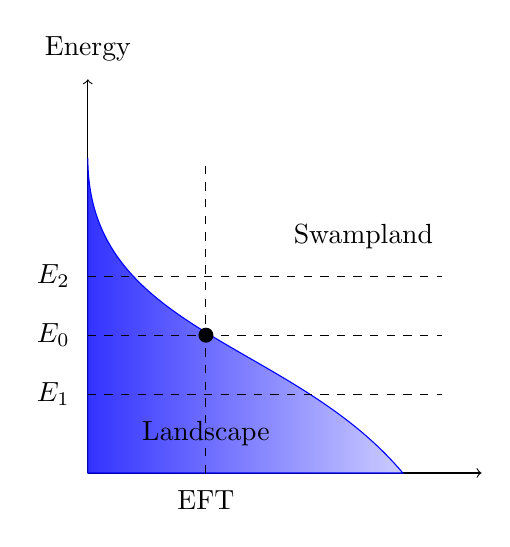
\begin{tikzpicture}[scale = 5]

        \draw[->] (0,0) -- (1,0);
        \draw[->] (0,0) -- (0,1) node[above=3pt]{Energy};
        \shadedraw[left color=blue!80!white,right color=blue!20!white, draw=blue] (0,0) -- (0,0.8) to [out=270, in=130] (0.8,0) -- cycle
        (0,0.2) node[left=3pt]{$E_{1}$}
        (0,0.5) node[left=3pt]{$E_{2}$}
        (0.3,0.1) node{Landscape}
        (0.7,0.6) node{Swampland};
        \draw[style=dashed] (0.3,0) node[below=3pt]{EFT} -- (0.3,0.8);
        \draw[style=dashed] (0,0.35) node[left=3pt]{$E_{0}$} -- (0.9,0.35);
        \draw[style=dashed] (0,0.2) -- (0.9,0.2);
        \draw[style=dashed] (0,0.5) -- (0.9,0.5);
        \filldraw[black](0.3,0.35) circle (0.5pt);
    \end{tikzpicture}
    \caption{This shows the cross section of figure \ref{fig:swampland}. Given an EFT at some lower energy scale, it belongs to the landscape as long as its characteristic energy is below $E_{0}$. However, the same EFT turns to be in the Swampland if the energy scale is above it. For instance, this EFT is in the landscape if it provides a description of physics of energy $E_{1}$, while it is in the Swampland if it does of $E_{2}$.}
    \label{fig:cross}
\end{figure}
Thus, whether an EFT belongs to the Swampland or the landscape is depending on at which energy scale it is used for an illustration of a physical system. As such energy increases, there are more strict constraints, and eventually the landscape gets smaller and smaller.\\
\indent To achieve concrete conditions which determine the boundaries between the Swampland and the landscape, phenomenological consequences, a lot of statements have been proposed. Those are called the Swampland conjectures.

\subsection{Swampland Conjectures}
At the moment, the Swampland conjectures are still proposals, not theorems because they have not been fully proven. That is why they are named conjectures. Yet, researches in recent years have found a large amount of evidence for some of them, and expectations that those conjectures might open the doors to the novel features of quantum gravity are increasing. Figure \ref{fig:connection} shows a map of conjectures as well as connections between them.
\begin{figure}
    \centering
    \begin{tikzpicture}
        \path[mindmap,concept color=black,text=white]
    node[concept] {No Global Symmetries}
    [clockwise from=0]
    child[concept color=green!50!black] {%
      node[concept](WG){Weak Gravity Conjecture}
      [clockwise from=0]
      child {node[concept] {Non-SUSY AdS Instability Conjecture} }
      %child {node[concept] {data structures} }
      %child {node[concept] {pro\-gramming languages} }
      %child {node[concept] {software engineer\-ing} }
    }  
    child[concept color=blue] {%
      node[concept](DC) {Swampland Distance Conjecture}
      [clockwise from=-30]
      child {node[concept] {No deSitter} }
      child {node[concept] {No Scale Separation in AdS} }
    }
    child[concept color=red] {node[concept] {Completeness Hypothesis} }
    child[concept color=orange] {node[concept] (TC){Trivial Cobordism} };
    \begin{pgfonlayer}{background}
        \draw [circle connection bar]
        (WG) edge (DC);
    \end{pgfonlayer}
    \end{tikzpicture}
    \caption{A schematic map of the Swampland conjectures}
    \label{fig:connection}
\end{figure}
In the following sections, only selected conjectures will be discussed in detail, which are most relevant for the purpose of the thesis. The connections between conjectures might indicate that some of them are equivalent statements with different appearances. Unifying them by better understanding of QG in the future is one of the goal of this area.

\section{No Global Symmetries in Quantum Gravity}
The absence of global symmetries is considered as the first Swampland conjecture, and widely accepted. Also, many of the Swampland conjectures can be considered as attempts to expand the idea that quantum gravity should have no global symmetries. The statement of the conjecture is as follows:
\begin{tcolorbox}[title=No Global Symmetries Conjecture,
    title filled=false,
    colback=blue!5!white,
    colframe=blue!75!black]
    There are no exact global symtries in quantum gravity.  %\textbf{tcolorbox}.
\end{tcolorbox} 
First of all, it is worth to recall briefly that a global symmetry is defined as an invariance under transformations described by a unitary operator commuting with the Hamiltonian. According to Noether's theorem, the continuous symmetry of a system indicates the existence of the conserved quantity, or charge, in it. For instance, the spatial translational symmetry leads to the conservation of momentum. There are a few kinds of arguments which support this conjecture. One motivation is from black hole physics. In order to illustrate what would make it invalid if a global symmetry is allowed in quantum gravity, assume that there \emph{is} an EFT coupled to gravity with a global symmetry. In the spectrum of EFT there are supposed to be states charged under such global symmetry. Suppose a black hole is charged by sending a charged state into it, it will evaporate decreasing its mass but maintaining its charge because Hawking radiation contains same number of positive/negative charged particles. Letting it evaporate completely, charge is supposed to vanish. Thus, it leads to a violation of the charge conservation. Also, even if such evaporation stops , and ends up with a remnant of mass $M \sim M_{P}$, since, according to the No-hair theorem, stable black holes can be distinguished from outside only by its mass, angular momentum, and gauge charge, it is impossible to determine its global charge given a black hole of a specific mass. Therefore, this process would violate charge conservations in a global symmetry as we started with non-zero charge and all the charge has disappeared after the evaporation of the black hole and no net charge has come out. Hence, in order to avoid this contradiction, it is necessary that global symmetries are forbidden in any theory of quantum gravity. This discussion can be extended to discrete symmetries and also to more generic global symmetries. Those are followed by the proposal of the Cobordism conjecture, which will be presented later.  \\
\indent The arguments above are rather motivation that proofs to grasp good intuitions for the conjecture. There are more formal evidences mainly from string theory. In particular, it is stated that there are no continuous global symmetry in the target space of perturbative string theory. Here we will briefly provide the proof for the case of bosonic string theory. For any global symmetry in the world sheet, we have a worldsheet charge given:
\begin{align}
    Q = \frac{1}{2\pi i} \oint (dzj_{z} - d\bar{z} j_{\bar{z}})
\end{align}
where $j_{z}$ and $j_{\bar{z}}$ are the symmetry currents. These char must be conformally invariant, and thus they transform as $(1,0)$, $(0,1)$ tensors respectively. Then we can build vertex operators in the forms:
\begin{align}
    j_{z}\bar{\partial} X^{\mu}e^{ikX} ,& \qq{} \partial X^{\mu} j_{\bar{z}}e^{ikX}
\end{align}
They create massless gauge vectors in the target space coupling to the left and right moving parts of the charge Q. Therefore, any global symmetry in the worldsheet turns into a gauge symmetry in the spacetime, and not to a global symmetry. So far, there is no counterexample of this conjecture. There is also a discussion through AdS/CFT and holography. A good reference for this evidence is . \\
\indent It is important to note that it is permitted that there is a low-energy theory with a global symmetry, as long as at higher energies such symmetry is gauged or broken. While it still gives understanding of the principles of quantum gravity, the No-global symmetries conjecture doesn't provide meaningful phenomenological constraints since nothing about at which scale such a global symmetry gets forbidden is stated. However, it is followed by other conjectures such as the Weak Gravity Conjectures and the Swampland Distance Conjecture, which give more concrete constraints, as expansions and refinements of the concept of the impossibility of exact global symmetries in quantum gravity. 


\section{Swampland Distance Conjecture}
The Swampland Distance Conjecture (SDC) is the one of the Swampland conjectures which give certain quantitative constraints. It provides a restriction on an EFT of quantum gravity when it is getting closer to where a global symmetry is restored. \\
\indent The motivation for the conjecture comes from the investigation in a moduli space, which is a space parametrized by the vacuum expectation value of some scalar fields. It is particular interest in that space to observe how an EFT changes as moving toward a certain direction where a global symmetry gradually is recovered, that is, some gauge coupling decreases to zero, because an exact global symmetry is not acceptable in quantum gravity. Therefore it is expected there is some phenomena in such limits in order to protect a theory to get back a global symmetry. One natural assumption to do so is that such poins are infinitely far away in a space. In addition, as an approximate global symmetry is getting exact as moving towards those limits, it is reasonable that an EFT is supposed to become an invalid description continuously. That is also predicted by the consequence of the Weak Gravity Conjecture. \\
\indent One important key point is that it is characteristic for a quantum gravity. Without considerring the quantum gravity, it is perfectly fine to have a point where a gauge coupling vanishes at infinite distance, and being close to it with maintaining a valid theory. Once the quantum gravity is taken into account, since taking a exact global symmetry strictly forbidden, an EFT should break down continuously as being closing to those limits. This can be generalized to other types of global symmetries. The Swampland Distance Conjecture provides information how EFT behaves when approaching infinite distance in a moduli space, and what features of quantum gravity makes it happen. 
\subsection{Moduli Space}
To begin with, let us clarify the notion of moduli space. For our purpose, the notion of moduli space denotes the space of different vacua. Suppose we have scalar fields $\phi ^{i}$, $i =1,\dotso ,n$, with a background and an effective action $\Gamma$. The expectation value of the scalar fields extremized this effective action, that is:
\begin{align}
    \fdv{\phi ^{i}} \Gamma (\expval{\phi ^{i}}) = 0
\end{align}
Once we find a quantum mechanically stable background, wee can study perturvation around such a background. Assume that the an effective action at low-energy regimes can be approximated with the action:
\begin{align}
    \Gamma = \int d^{d}x \lbrace \frac{1}{2} g_{ij} \partial _{\mu} \phi ^{i} \partial ^{\mu} \phi ^{j} - V_{\text{eff}} (\phi ^{i}) \rbrace
\end{align}
plus terms with fields other than scalars. Now we want to find values of scalar fields which make the potential minimum. This is not necessarily a single point, but can be a manifold. Because the potential remains constant in the direction of field space that potential stays minimum, they are called the flat directions of the field space. Let us assume the minimum value of the potential is zero. \\
\indent The subspace where $V_{\text{eff}} = 0$ of the field space is called the moduli space and it represents the space of different vacua. Assuming the moduli space is parametrized by the vacuum expectation values of scalar fields $\phi ^{I}$. The kinetic term for those scalar fields takes the form as following:
\begin{align}
    \int d^{d}x \frac{1}{2} g_{IJ} (\phi) \partial _{\mu} \phi ^{I} \partial ^{\mu} \phi ^{J}  
\end{align}
where $g_{IJ}$ can be thought of as a metric on the field space. This action is apparently the non-linear sigma model. Using this metric, we can compute geometric quantities associated with this moduli space such as the geodesic distance and volume.
\subsection{preliminary Introduction to String Theory}
Since the Distance conjecture is closely related to the string theory, it is essential to provide the basic introduction to it. It will be based on familiar discussions covered by standard textbooks for the string theory.
\subsubsection{The Nambu-Goto Action}
Consider a point particle and assume it propagates in D-dimensional spacetime $\mathbb{R}^{1,D-1}$. We can assign the coordinates as $X^{0} = t$ and $X^{i}$, with $i = 1, \dotso , D-1$ for the description of the motion of the particle. Then its motion is associated to a world-line $\gamma$ which identify $X^{i} (X^{0})$. Also the particle world-line in relativistic coordinates can be described by a world-line parameter $\tau$ so that $\gamma$ specifies $X^{\mu}(\tau)$, where $\mu = 0,1,\dotso , D-1$ :
\begin{align}
    \gamma : \tau \hookrightarrow X^{\mu} (\tau) \in \mathbb{R} ^{1,D-1}
\end{align}
\begin{figure}
    \centering
    \begin{tikzpicture}[scale=5]
        \draw[->] (0,0) -- (1,0) node[right=1pt]{$X^{i}$};
        \draw[->] (0,0) -- (0,1) node[left=2pt] {$X^{0}$};
        \draw[->, red] (.5,.2) .. controls (.8,.4) .. (.7,.5) node[right=2pt,black] {$\tau$};
        \draw[red] (.7,.5) .. controls (.5,.8) .. (.75,.9);
        \draw[->, blue!70] (.8,.8) node[right=3pt,black]{world-line, $\gamma$} -- (.65,.65);
    \end{tikzpicture}
    \caption{Illustration of the world-line of a moving particle.}
    \label{fig:worldline}
\end{figure}
Figure \ref{fig:worldline} shows the description of the particle motion. \\
\indent In Minkowski space, the line element is given:
\begin{align}
    ds^{2} = \eta_{\mu \nu} dX^{\mu} dX^{\nu} 
\end{align}
Then we can write an action for a particle, which can be simply written as the length of time-like world-line:
\begin{align}
    S_{\text{NG}} = -m\int _{\gamma} \sqrt{-ds^{2}} = -m\int _{\gamma} (-\dot{X}^{2})^{1/2} d\tau
\end{align}
where $\dot{X} ^{\mu} = \pdv{X^{\mu}}{\tau}$, $\dot{X} ^{2} = \eta _{\mu \nu} \dot{X}^{\mu} \dot{X} ^{\nu}$, and m is a constant related to the mass of the particle. This action is called the Nambu-Goto action. Consider a Lagrangian:
\begin{align}
    S_{\text{NG}} = -m\int_{\gamma} d\tau L(\tau)
\end{align}
The canonical momentum is:
\begin{align}
    p_{\mu} = \pdv{L}{\dot{X}^{\mu}} = \frac{m\dot{X}_{\mu}}{(-\dot{X}^{2})^1/2}
\end{align}
Then it ends up with a constraint:
\begin{align}
    p^{2} + m^{2} = 0
\end{align}
which illustrates that m is actually the mass of the particle. The equation of motion for $X^{\mu}$ gives:
\begin{align}
    m\ddot{X}^{\mu} =0
\end{align}
then we can see that the action is correctly describing the free propagation of the particle.
\subsubsection{The Polyakov Action}
We can suppose another action for a particle which is called the Polyakov action given:
\begin{align}
    S_{P} = \frac{1}{2} \int _{\gamma} d\tau e(\tau) \lbrace \frac{1}{e(\tau)^{2}} \dot{X}^{2} - m^{2} \rbrace
\end{align}
$e(\tau)$ is named the world-line metric. The equation of motion corresponding to this action is:
\begin{align}
    \dot{X}^{2} + m^{2} e(\tau) ^{2} =0
\end{align}
Using it, we can deform the Polyakov action by eliminating the world-line metric:
\begin{align}
    S_{P} = \frac{1}{2} \int _{\gamma} d\tau e(\tau) (-2m^{2}) = -m \int _{\gamma} d\tau(-\dot{X}^{2})^{1/2} = S_{\text{NG}}
\end{align}
Therefore, the Nambu-Goto action and the Polyakov action are equivalent to each other. The reason we use the polyakov action is that it is much easier to quantize.
\subsubsection{The String Worldsheet}
Let us do the same computations, but now we are dealing with a string, not a particle. Considering the motion of a string, it sweeps out a 2-dimensional worldsheet $\Sigma$ parametrized by two coordinates $(\sigma, \tau)$:
\begin{align}
    \Sigma : (\sigma,\tau) \hookrightarrow X^{\mu} (\sigma, \tau) \in \mathbb{R} ^{1,D-1}
\end{align}
Define the ranges:
\begin{align}
    0 \le \sigma \le 2\pi, & \qq{} \tau \in \mathbb{R}
\end{align}
SInce we are mostly interested in closed strings, rather than open ones, we impose the boundary condition given:
\begin{align}
    \sigma \simeq \sigma + 2\pi
\end{align}
So the string worldsheet parametrized by such coordinates forms a cylinder as shown in figure \ref{fig:worldsheet}.
\begin{figure}
    \centering
    \begin{tikzpicture}[scale=5pt]
        \draw[->] (0,0) -- (1,0) node[right=1pt]{$X^{i}$};
        \draw[->] (0,0) -- (0,1) node[left=2pt] {$X^{0}$};
        \node[cylinder, draw, shape aspect=.5, 
      cylinder uses custom fill, cylinder end fill=green!50, 
      minimum height=1cm,
      minimum width=0.5cm,
      cylinder body fill=green!25, opacity=0.5, 
    scale=3, rotate=90](c) at (.5,.5) {};
    \draw[->,red] (.5,.84) -- (.52,.84) node[above=1pt,black] {$\sigma$};
    \draw[->, red] (.65,.5) -- (.65,.5) node[right=1pt, black] {$\tau$};
    \draw[->, green] (.9,.8) node[right=2pt, black]{worldsheet $\Sigma$}-- (.7,.7); 
    \end{tikzpicture}
    \caption{The worldsheet of a string parametrized by two coordinates $(\sigma, \tau)$}
    \label{fig:worldsheet}
\end{figure}
It is useful to denote the coordinates as:
\begin{align}
    \lbrace \sigma, \tau \rbrace \equiv \xi ^{a}, & \qq{} a=0,1
\end{align}
With the worldsheet metric $h_{ab} (\xi)$, the string tension $T$ which can be written in terms of a parameter $\alpha '$:
\begin{align}
    T \equiv \frac{1}{2\pi \alpha '}    
\end{align}
the Polyakov actions for the string is given:
\begin{align}
    \label{eq:1.20}
    S_{P} = -\frac{T}{2} \int _{\Sigma} d^{2} \xi (-\text{det} h) ^{1/2} h^{ab} (\xi) \eta _{\mu \nu} \partial _{a} X^{\mu} (\xi) \partial _{b} X^{\nu} 
\end{align}
Besides, there are also the string length $l_{s}$ and the string scale $M_{s}$, given:
\begin{align}
    l_{s} \equiv \sqrt{\alpha '} , & \qq{} M_{s} \equiv \frac{1}{2\pi \sqrt{\alpha '}}
\end{align}
The worldsheet action eq\ref{eq:1.20} should be viewed as a description of a two-dimensional theory with scalars $X^{\mu} (\xi)$, which is the sigma model. The space-time parametrized by $X^{\mu} (\xi)$ is known as the target space of the theory. The metric $\eta _{\mu \nu}$ on the space-time is the metric on the field space of the scalar fields $X^{\mu}$. Therefore, there are supposed to be different metrics on the field spaces for different target spaces in which strings propagate.
\subsubsection{Symmetries on the Worldsheet}
Eq \ref{eq:1.20} is invariant under:
\begin{align}
    \xi ^{a} \rightarrow \tilde{\xi} ^{a} (\xi)
\end{align}
In addition, it is invariant under the Weyl transformation given:
\begin{align}
    \delta X^{\mu} = 0, & \qq{} h_{ab} \rightarrow \tilde{h}_{ab} = e^{2\Lambda (\xi)} h_{ab}
\end{align}
The symmetries are useful for fixing the worldsheet metric $h_{ab}$. For D-dimensional theory, each number of degrees of freedom in the metric, a symmetric tensor, and so on. Particulaely, the number of degrees of freedom in $h_{ab}$ is $\frac{1}{2}D(D+1)$, and for a string, $D=2$, the number of symmetry parameters is the same as the degrees of freedom in the metric. With symmetries, we can after all get:
\begin{align}
    h_{ab} = \eta _{ab} = 
    \begin{bmatrix}
        -1 & 0 \\
        0 & 1
    \end{bmatrix}
\end{align}
which is called flat gauge. Notice that it is still necessary to have equations of motion while the metric can be gaged. The equation of motion for the metric corresponding to the vanishing of the energy momentum tensor is:
\begin{align}
    T_{ab} =0
\end{align}
where:
\begin{align}
    T_{ab} \equiv \frac{4\pi}{\sqrt{-\text{det} h}} \fdv{S_{P}}{h^{ab}}
\end{align}
This is called a Virasoro constraint, and plays important role for the quantization of the string. \\
\indent In flat gauge, the reduced Polyakov action is:
\begin{align}
    S_{P} = \frac{T}{2} \int _{\Sigma} d\sigma d\tau \lbrace (\partial _{\tau} X)^{2} - (\partial _{\sigma} X)^{2}  
\end{align}
Now we can go to light-cone coordinates:
\begin{align}
    \xi ^{\pm} \equiv \tau \pm \sigma, & \qq{} \partial _{\pm} \equiv \frac{1}{2} (\partial _{\tau} \pm \partial _{\sigma})
\end{align}
Then the action deforms:
\begin{align}
    S_{P} = T\int _{\Sigma} d\xi ^{+} d\xi ^{-} \partial _{+} X \partial _{-} X
\end{align}
The equation of motion therefore for $X^{\mu}$ are:
\begin{align}
    \partial _{+} \partial _{-} X^{\mu} = 0
\end{align}
Thus $X^{\mu}$ can be thought of as the sum of left- and right-mooving parts of the strings as:
\begin{align}
    X^{\mu} = X_{L} ^{\mu} (\xi ^{+}) + X_{R} ^{\mu} (\xi ^{-})
\end{align}
Also considering the periodic boundary conditions $X^{\mu} (\tau, \sigma = 0) = X^{\mu} (\tau, \sigma = 2n\pi)$, the most general solution is:
\begin{align}
    \begin{split}
        & X_{R} ^{\mu} (\xi ^{-}) = \frac{1}{2} (x^{\mu}) +c^{\mu}) + \frac{1}{2}\alpha' p_{R} ^{\mu}\xi ^{-} + i\sqrt{\frac{\alpha'}{2}}\sum_{n\in\mathbb{Z}, n\neq 0} \frac{1}{n}\alpha_{n}^{\mu} e^{-in\xi^{-}} \\
        & X_{L} ^{\mu} (\xi ^{+}) = \frac{1}{2} (x^{\mu}) -c^{\mu}) + \frac{1}{2}\alpha' p_{L} ^{\mu}\xi ^{+} + i\sqrt{\frac{\alpha'}{2}}\sum_{n\in\mathbb{Z}, n\neq 0} \frac{1}{n}\tilde{\alpha}_{n}^{\mu} e^{-in\xi^{+}}
    \end{split}
\end{align}
where $x^{\mu}$, $c^{\mu}$, $p_{R}^{\mu}$, $p_{L}^{\mu}$, $\alpha _{n} ^{\mu}$, $\tilde{\alpha} _{n} ^{\mu}$ are constants. Due to the periodicity:
\begin{align}
    p_{R}^{\mu} = p_{L}^\mu \equiv p^{\mu}
\end{align}
Averaging over the string, one may find:
\begin{align}
    q^{\mu} \equiv \frac{1}{2\pi} \int _{0} ^{2\pi} d\sigma X^{\mu} = x^{\mu} + \alpha'p^{\mu} \tau
\end{align}
Thus we can say that $x^{\mu}$ is the center of mass position, and $p^{\mu}$ is the target space momentum. 
\subsubsection{Spectrum}
Considerations so far have been in classical manner, but it is needed to quantize strings in order to investigate the spectrum of excitations. In the following, we will manipulate so-called light-cone quantization. Introduce target-space light-cone coordinates:
\begin{align}
    X^{\pm} \equiv \frac{1}{\sqrt{2}} (X^{0} \pm X^{D-1}), & \qq{} X^{i}, & \qq{} i = 1,\dotso ,D-2
\end{align} 
Then the metric takes the form:
\begin{align}
     \eta _{+-} = \eta {-+} = -1, & \qq{} \eta _{oj} = \delta _{ij}
\end{align}
With this, an inner product is defined:
\begin{align}
    X^{2} = -2X^{+}X^{-} + \dot {X}^{i} \dot {X}^{i}
\end{align}
The expansion of $X^{+}$ is:
\begin{align}
    X^{+} (\tau,\sigma) = x^{+} + \alpha' p^{+} \tau + i\sqrt{\frac{\alpha'}{1}} \sum _{n\in \mathbb{Z},n\neq 0} \frac{1}{n} \alpha _{n} ^{+} e^{-in\xi ^{-}} +i\sqrt{\frac{\alpha'}{1}} \sum _{n\in \mathbb{Z},n\neq 0} \frac{1}{n} \tilde{\alpha} _{n} ^{+} e^{-in\xi ^{+}}
\end{align}
Since there are residual symmetries even if we choose the light-cone gauge, we can set all the oscillator modes of $X^{+}$ to zero. Then:
\begin{align}
    X^{+} (\tau,\sigma) = x^{+} + \alpha'p^{+}\tau
\end{align}
Imposing the Virasoro constraints as well:
\begin{align}
    \partial _{\pm} X^{-} = \frac{1}{\alpha' p^{+}} (\partial _{\pm} X^{i})^{2}
\end{align}
We can observe that the $X^{-}$ oscillators are written in the transverse oscillators in $X^{i}$ too. Therefore, only the transverse oscillators are independent degrees of freedom. This is very useful because only $X^{i}$ contains physically independent oscillators and rules out tow unphysical polarizations of the string. The action in the light-cone gauge becomes:
\begin{align}
    S_{LC} &= \frac{1}{4\pi \alpha'} \int _{\sigma} d\tau d\sigma \lbrace (\partial _{\tau} X^{i})^{2} - (\partial _{\sigma} X^{i})^{2} + 2(\partial _{\sigma} X^{+} \partial _{\sigma} X^{-} - \partial _{\tau} X^{+} \partial _{\tau} X^{-}) \rbrace \nonumber \\
    &= \frac{1}{4\pi\alpha'} \int _{\sigma} d\tau d\sigma \lbrace (\partial _{\tau} X^{i})^{2} - (\partial _{\sigma} X^{i})^{2} - \int d\tau p^{+} \partial _{\tau} q^{-} \nonumber \\
    & \equiv \int d\tau L 
\end{align}
where defined as:
\begin{align}
    q^{-} \equiv \frac{1}{2\pi} \int _{0} ^{2\pi} d\sigma X^{-}
\end{align}
From this, canonical momenta are given:
\begin{align}
    p_{-} \equiv \pdv{L}{\dot{q}^{-}} = -p^{+}, & \qq{} \Pi _{i} \equiv \pdv{L}{\dot{X}^{i}}= \frac{\dot{X}_{i}}{2\pi \alpha'}
\end{align}
Then quantize the theory by introducing the canonical commutaion relations:
\begin{align}
    [X^{\mu}(\tau,\sigma), \Pi^{\mu} (\tau,\sigma;)] = i\eta ^{\mu \nu} \delta(\sigma - \sigma')
\end{align}
followed by:
\begin{align}
    [x^{i},p^i] &= i\delta_{ij}, \\
    [p^{+},q^{-}] &= i, \\
    [\alpha _{m}^{i},\alpha _{n}^{j}] &= m\delta_{m+n,0}\delta_{ij},\\
    [\tilde{\alpha}_{m}^{i}, \tilde{\alpha}_{n}^{j}] &= m\delta_{m+n,0} \delta_{ij} 
\end{align}
Then we can adopt the standard procedure of quantization by promoting the oscillator modes to operators acting on a Hilbert space as in QFT. In this case, $\alpha_{-n} ^{i}$ with $n>0$ are creation operators acting on a vacuum state $\ket{0,p}$. On the other hand $\alpha_{n}^{i}$ with $n>0$ represent annihilation operators. Recall that there are no oscillators to quantize for $X^{+}$, while the $X^{-}$ oscillators are given in terms of $X^{i}$. Explicitly:
\begin{align}
    \alpha _{n}^{-} = \frac{1}{2p^{+}\sqrt{2\alpha'}} \sum _{m=-\infty} ^{m=\infty} \alpha _{n-m} ^{i} \alpha _{m} ^{i}
\end{align}
Since the ordering of the $\alpha$ matters, we need the notions of normal ordered products and a normal ordering constant a where:
\begin{align}
    \alpha_{n} ^{-} = \frac{1}{2p^{+} \sqrt{2\alpha'}} \left( \sum_{m=-\infty} ^{m=\infty} :\alpha_{n-m}^{i} \alpha_{m}^{i}: -a\delta_{n,0} \right) 
\end{align}
with the definition:
\begin{align}
    :\alpha_{m}^{i} \alpha_{n}^{i}: \equiv 
    \begin{cases}
        \alpha_{m}^{i} \alpha_{n}^{i} & \quad \text{for } m \leq n \\
        \alpha_{n}^{i} \alpha_{m}^{i} & \quad \text{for } n < m 
    \end{cases}
\end{align}
\subsubsection{Lorentz Invariance}
So far we have performed quantization in special target-space light-cone coordinates. So we should also think about Lorentz invariance in the theory. Generally, the generators of the Lorentz transformations are given:
\begin{align}
    J^{\mu \nu} = \int _{0}^{2\pi} d\sigma (X^{\mu} \Pi ^{\nu} - X^{\nu} \Pi ^{\mu}) \equiv l^{\mu\nu} + E^{\mu\nu}+ \tilde{E}^{\mu\nu}
\end{align}
where
\begin{align}
    l ^{\mu\nu} &= x^{\mu} p^{\nu} - x^{\nu}p^{\mu} \\
    E^{\mu\nu} &= -i\sum_{n=1}^{\infty} \frac{1}{n} (\alpha_{-n}^{\mu}\alpha_{n}^{\nu} - \alpha_{-n}^{\nu} \alpha_{n}^{\mu}) \\
    \tilde{E^{\mu\nu}} &= -i\sum_{n=1}^{\infty} \frac{1}{n} (\tilde{\alpha}_{-n}^{\mu}\tilde{\alpha}_{n}^{\nu} - \tilde{\alpha}_{-n}^{\nu} \tilde{\alpha}_{n}^{\mu})
\end{align}
Lorentz algebra reads:
\begin{align}
    [J^{\mu\nu}, J^{\rho\sigma}] = i\eta ^{\mu\rho}J^{\nu\sigma} + i\eta^{\nu\sigma}J^{\mu\rho} - i\eta^{\mu\sigma}J^{\nu\rho} - i\eta^{\nu\rho}J^{\mu\sigma}
\end{align}
Particularly:
\begin{align}
    [J^{-i},J^{j}] = 0
\end{align}
but at the same time, this calculation followed by:
\begin{align}
    [J^{-i},J^{-j}] = -\frac{1}{(p^{+})^{2}} \sum_{m=1}^{\infty} \lbrace \frac{26-D}{12}m + \frac{1}{m}(\frac{D-26}{12} + 2(1-a))(\alpha_{-m}^{i} \alpha_{m}^{j} - \alpha_{-m}^{j} \alpha_{m}^{i}) + (\text{tilde terms}) 
\end{align}
So for the Lorentz invariance at quantum level, there are constraints such as:
\begin{align}
    D=26, & \qq{} a=1
\end{align}
It claims that the quantum bosonic string is only consistent in 26-dimensions. Such a restricion on the dimensionality is named criticality. Note that this is the case for the bosonic string, and for the superstring, the number of dimensions is 10.

\subsubsection{Quantum String Spectrum}
Let us study the spectrum of the quantized string. The Hamiltonian is:
\begin{align}
    \begin{split}
    H &= p_{-} \dot{q}^{-} +\int _{0}^{2\pi} d\sigma \Pi _{i} \dot{X}^{i} - L \\
    &=\frac{1}{4\pi\alpha'} \int_{0}^{2\pi}d\sigma  \left[ (\partial_{\tau} X^{i})^{2} + (\partial _{\sigma} X^{i})\right] \\
    &= \frac{\alpha'}{2}p^{i}p^{i} + \frac{1}{2} \sum_{n=-\infty}^{\infty} (\alpha_{-n}^{i} \alpha_{n}^{i} + \tilde{\alpha}_{-n} ^{i} \tilde{\alpha} _{n}^{i})
    \end{split}
\end{align}
From the Virasoro constraint:
\begin{align}
    \partial _{\tau} X^{-} = \frac{1}{2p^{+}\alpha'} \left[ (\partial_{\tau}X^{i})^{2} + (\partial _{\sigma} X^{i})^{2}\right]
\end{align}
we may have:
\begin{align}
    p^{-} = \frac{1}{2\pi\alpha'}\int_{0}^{2\pi} d\sigma \partial _{\tau} X^{-} = \frac{H}{\alpha' p^{+}}
\end{align}
Considering normal ordering of $\alpha$:
\begin{align}
    p^{+}p^{-} = \frac{1}{\alpha'} \left[ \sum_{n=1} ^{\infty} :\alpha _{-n}^{i} \alpha_{n}^{i}: + \sum_{n=1}^{\infty} :\tilde{\alpha}_{-n}^{i} \tilde{\alpha} _{n}^{i}: -2a + \frac{\alpha'}{2}p^{i}p^{i} \right]
\end{align}
The mass in the target space is:
\begin{align}
    M^{2} = -p^{2} = 2p^{+}p^{-} -p^{i}p^{i} = \frac{2}{\alpha'} \left[ \sum_{n=1} ^{\infty} :\alpha _{-n}^{i} \alpha_{n}^{i}: + \sum_{n=1}^{\infty} :\tilde{\alpha}_{-n}^{i} \tilde{\alpha} _{n}^{i}: -2a \right]
\end{align}
But for the closed string there is a symmetry regarding translations along $\sigma$ implying the level matchong condition:
\begin{align}
    \sum_{n=1} ^{\infty} :\alpha _{-n}^{i} \alpha_{n}^{i}: = \sum_{n=1}^{\infty} :\tilde{\alpha}_{-n}^{i} \tilde{\alpha} _{n}^{i}:
\end{align}
this leads to the mass expression in:
\begin{align}
    M^{2} = \frac{4}{\alpha'} (\sum_{n=1} ^{\infty} :\alpha _{-n}^{i} \alpha_{n}^{i}: -1)
\end{align}
applying the criticality to fix $a=1$. Now we can start to study the spectrum. Let us define $\sum_{n=1} ^{\infty} :\alpha _{-n}^{i} \alpha_{n}^{i}: = N$. \\
For $N=0$ case, we have:
\begin{align}
    M^{2}= -\frac{4}{\alpha'}
\end{align}
This is a tachyonic mode and suggesting an instability in the bosonic string. \\
For $N= 1$:
\begin{align}
    M^{2}=0
\end{align}
So it is the massless spectrim, and given by:
\begin{align}
    \xi _{ij} \tilde{\alpha}_{-1}^{i} \alpha_{-1}^{j} \ket{0,p}, & \qq{} i,j=1.\dotso ,24
\end{align} 
The tensor $\xi_{ij}$ can be decomposed into irreducible representations of SO(24):
\begin{align}
    \xi _{ij} = g_{(ij)} + B_{[ij]} + \Phi
\end{align}
where $g_{(ij)}$ and $B_{[ij]}$ are traceless symmetric and anti-symmetric respectively as well as $\Phi$ represents a scalar. Thus we obtain a massless, transversely polarized symmetric tensor fields $g_{ij}$, which is a graviton. Therefore the quantum string contains gravitational modes in spectrum. \\
For $N>1$, we may have massive oscillator string modes.

\subsection{Realization of the Distance Conjecture}
We have found that the bosonic string lives in 26-dimensions, and mentioned the superstring does in 10-dimension. Those facts seem to make them incompatible directly with the observed universe. Nevertheless, they can be observed yet since the addtional dimensions might be compact and small. In this language, it is naturall to thinka about string theory in a spacetime which has a compact direction. One of possible settings is the case where one of the dimensions is in the form of a circle. Studying this, we will see a realization of the Distance conjecture.

\subsubsection{Compactification on a Circle}
Consider $D=d+1$ dimensional spacetime. Let the spatial direction $X^{d}$ to be compact in the shape of a circle with periodicity:
\begin{align}
    X^{d} \simeq X^{d} +1
\end{align}
notice that we are working in Planck units, so the periodicity is set to one. \\
\indent The metric on the D-dimensional space is given:
\begin{align}
    \label{eq:met}
    ds^{2} \equiv G_{MN} dX^{M}dX^{N} = e^{2\alpha\phi}g_{\mu\nu} dX^{\mu}dX^{\nu} + e^{\beta\phi}(dX^{d})^{2}
\end{align}
There some coordinates and parameters are introduced. Coordinates $X^{M}$ are D-dimensional, $M=0, \dotso , d$, while $\mu = 0, \dotso ,d-1$. The D-dimensional metric is $G_{MN}$, and d-dimensional one is $g_{\mu\nu}$. The metric has a parameter $\phi$ which represents a d-dimensional scalar field. In addition, the constants $\alpha$ and $\beta$ have been defined:
\begin{align}
    \alpha^{2} = \frac{1}{2(d-1)(d-2)} , & \qq{} \beta = -(d-2) \alpha
\end{align}
The circumference of the circle denoted $2\pi R$ is:
\begin{align}
    \label{eq:circ}
    2\pi R \equiv \int _{0}^{1} \sqrt{G_{dd}}dX^{d} = e^{\beta\phi}
\end{align}
Then the radius is a dynamical field in d-dimensions. Our interest will be in the behaviors of the d-dimensional theory under variations of the expectation value of the field $\phi$, which amounts to variations of the size of the circle. \\
\indent Consider the decomposition of the D-dimensional Ricci scalar $R^{D}$ for the metric \ref{eq:met}. We have:
\begin{align}
    \label{eq:eff}
    \int d^{D}X \sqrt{-G} R^{D} = \int d^{d}X \sqrt{-g} \left[R^{d} -\frac{1}{2} (\partial \phi)^{2} \right]
\end{align}
Introduce a massless D-dimensional scalar field $\Psi$. Due to the periodicity:
\begin{align}
    \Psi (X^{M}) = \sum_{n=-\infty}^{\infty} \psi_{n} (X^{\mu}) e^{2\pi i n X^{d}}
\end{align}
The modes $\psi _n$ are d-dimensional scalar fields caleld Kaluza-Klein (KK) modes, and $\psi _{0}$ is the zero-mode of $\Psi$. The momentum is quantized along the compact direction:
\begin{align}
    -i\pdv{X^{d}} \Psi = 2\pi n \Psi
\end{align}
Now to make things simple, assume $g_{\mu\nu} = \eta _{\mu\nu}$. The equation of motion for $\Psi$ is:
\begin{align}
    \partial ^{M} \partial _{M} \Psi = (e^{-2\alpha \phi} \partial ^{\mu} \partial _{\mu} + e^{-2\beta \phi} \partial _{X^{d}}^{2}) \Psi = 0
\end{align}
since $\Psi$ is massless. Then this leads the equation of motion for $\psi _n$ modes:
\begin{align}
    \left[\partial ^{\mu}\partial _{\mu}- (\frac{1}{2\pi R})^{2} (\frac{1}{2 \pi R})^{\frac{2}{d-2}} (2\pi n)^{2}  \right] \psi _{n} = 0
\end{align}
Therefore, the mass of the KK modes can be read off as:
\begin{align}
    M_{n} ^{2}= (\frac{n}{R})^{2} (\frac{1}{2 \pi R})^{\frac{2}{d-2}}
\end{align}

\subsubsection{Compactification of String on a Circle}
Now let us do the same procedure in the string theory considering strings on a circle of radius R. A metric is given:
\begin{align}
    \label{eq:metric}
    ds^{2} = \eta _{MN} dX^{M} dX^{N}
\end{align}
taking the $X^{d}$ direction as R-periodic:
\begin{align}
    X^{s} \simeq X^{d} + 2\pi R
\end{align}
Consider the bosonic mode expansion as before but for now, we will not impose $X^{M} (\sigma + 2\pi, \tau) = X^{M} (\sigma,\tau)$. Thus:
\begin{align}
    X^{M} (\tau, \sigma) = x^{\mu} + \alpha' p^{M} \tau + \frac{\alpha'}{2}(p_{L}^{M} - p_{R}^{M}) \sigma + \text{oscillator}
\end{align}
Here left- and right mooving momenta are considered independently, and the overall momentum is:
\begin{align}
    \frac{1}{2} (p_{R}^{M} + p_{L} ^{M})
\end{align}
In the non-compact space, imposing $X^{\mu} (\sigma+2\pi, \tau) = X^{\mu}(\sigma,\tau)$, we have $p_{R}^{\mu} = p_{L}^{\mu}$. However, for a circle we have a winding:
\begin{align}
    X^{d} (\sigma +2\pi, \tau) = X^{d} (\sigma,\tau) + w 2\pi R ,& \qq{} w \in \mathbb{Z}
\end{align}
The string is wrapping around a circle w times. Therefore, we may have:
\begin{align}
    \frac{\alpha'}{2} (p_{L}^{d} - p_{R}^{d}) =wR
\end{align}
Consider the mass spectrum for the string by going to target space light-cone gauge again. The hamiltonian reads:
\begin{align}
    H = \frac{\alpha'}{2} \left[ \frac{1}{4} (p_{L}^{d} -p_{R}^{d})^{2} +p^{\alpha} p^{\alpha} + (p^{d})^{2} \right] + (N + \tilde{N} -2)
\end{align}
here we split the index $i = \lbrace \alpha, d \rbrace$. Notice in this case we no longer have the level matching condition, but instead:
\begin{align}
    N-\tilde{N} = nw
\end{align} 
Then the d-dimensional mass is given by $-p_{\mu} p^{\mu} = 2p^{+} p^{-} - p^{\alpha} p^{\alpha}$ which leads:
\begin{align}
    \label{eq:1.90}
    (M_{n,w})^{2} = (\frac{n}{R})^{2} + (\frac{wR}{\alpha'})^{2}
\end{align}
We want to make it related to the effectiveaction \ref{eq:eff}. Nevertheless, we need to change form the metric \ref{eq:metric} to the one \ref{eq:met}. This procedure is called going from the string frame to the Einstein frame. The difference is the factor of $E^{2\alpha\phi}$ multiplying the $g_{\mu\nu}$ directions. An important object is the d-dimensional scalar $\Psi$, called dilaton, defined as:
\begin{align}
    \Psi^{d} \equiv \Psi - \frac{1}{2} \log (2\pi R M)
\end{align}
We would like to observe variations of R which maintain $\Psi ^{d}$ fixed. That is, we must vary:
\begin{align}
    e^{2\Psi} \sim \frac{1}{2\pi R M}
\end{align}
But considering the definition of the d-dimensional Planck mass $M_{p}^{d}$:
\begin{align}
    \frac{(M_{p}^{d})^{d-2}}{2} \equiv 2\pi M^{D-2} e^{-2\Psi}
\end{align}
From this we can see that in order to remain the Einstein frame $M_{p} ^{d} = 1$, we must choose our units so that:
\begin{align}
    M \sim (2\pi R) ^{\frac{1}{d-2}}
\end{align}
This affects the mass of the winding modes in \ref{eq:1.90}. \\
\indent Finally, performing the change of frames leads to the Einstein frame mass:
\begin{align}
    \label{eq:efram}
    (M_{n,w})^{2} = (\frac{1}{2\pi R})^{\frac{2}{d-2}} (\frac{n}{R})^{2} + (2\pi R)^{\frac{2}{d-2}} (\frac{wR}{\alpha_{0}'})^{2}
\end{align}

\subsubsection{Distance Conjecture}
We will now study the d-dimensional effective theory. The action is given in \ref{eq:eff} and this has to be supplemented by the spectrum \ref{eq:efram}. Our particular interest is how the spectrum of states behaves under variations of the expectation value of the field $\phi$. This can be determined easily from the relation \ref{eq:circ}. The possible expectation values of the field $\phi$ define a field space $\mathcal{M}_{\phi}$, which has now one infinite real dimension. Thus consider:
\begin{align}
    \mathcal{M}_{\phi} : -\infty < \phi < \infty
\end{align}
We are now having two infinite towers of massive states in this theory, in eq \ref{eq:efram}, the tower of KK modes with masses $M_{n,0}$, and of winding modes with $M_{0,m}$. Using the relation \ref{eq:circ}, those mass scales can be written as:
\begin{align}
    M_{\text{KK}} \sim E^{\alpha\phi}, & \qq{} M_{w} \sim e^{-\alpha \phi}
\end{align}
where
\begin{align}
    \alpha = \sqrt{2} (\frac{d-1}{d-2})^{1/2} > 0
\end{align}
For any variation $\Delta \phi$ there exists an infinite tower of states with associated mass scale M. We can also see that such a tower becomes light at an exponential rate in $\Delta \phi$:
\begin{align}
    \label{eq:mass}
    M(\phi_{i} + \Delta \phi) \sim M(\phi _{i})e^{-\alpha \abs{\Delta \phi}}
\end{align}
as illustrated in figure \ref{fig:dual}.
\begin{figure}
    \centering
    \begin{tikzpicture}[scale=5]
        \draw[->] (-0.7,0) node[below=2pt] {$-\infty$} -- (0.7,0) node[below=2pt] {$+\infty$};
        \draw[->] (0,-.5) -- (0,0.5) node[left=2pt] {$\ln \frac{M}{M_{p}}$};
        \draw[blue] (-0.6,-0.4) -- (0.6,0.4) node[above=2pt,black] {$M_{KK}$};
        \draw[red] (-.6,0.4) node[above=2pt, black] {$M_{w}$} -- (0.6,-0.4);
    \end{tikzpicture}
    \caption{Illustration of the mass scales on a log plot. For the KK and winding towers as a function of the scalar field $\phi$ expectation value.}
    \label{fig:dual}
\end{figure}
There are a few things to note:
\begin{itemize}
    \item {The tower of states becoming light is the KK tower if $\Delta \phi <0$ while it is the winding tower when $\Delta \phi >0$. That is, either tower of states always becomes light regardless of the sign of $\Delta\phi$ is.}
    \item {This is a characteristic feature of the string theory. It is not true in QFT since winding states are absent in field theories.}
    \item {The product of the mass scales of the two towers is independent of $\phi$.}
    \item {The exponent $\alpha$ is a constant of order one $\order{1}$.}
    \item {When $\abs{\Delta \phi} \rightarrow  \infty$, an infinite number of states get massless.} 
\end{itemize}
The last point has a discussion. If we consider an effective field theory which has a cut-off $\Lambda$ below the mass scale of an infinite tower of states. Thus, this teory can be valid only for a finite range of expectation values of $\phi$. \\
\indent The exponential behavior is particularly interesting. Those towers are deeply related to each other as there is a $\mathbb{Z}_{2}$ symmetry which interchanges them. This relation is called T-duality, and it is able to be seen directly in the string frame where the mass spectrum is invariant under the action. 
\begin{align}
    \text{T-duality} : R \Leftrightarrow \frac{\sqrt{\alpha'}}{R}
\end{align}
Actually, it is a symmetry not only for the mass, but also for the full string theory. There are many other kinds of dualities other than T-duality. Then it is natural to think that there are many different towers of states which are dual so that as one moves in a space of the theory, the product of the mass scale of the dual towers remains constant and thus one must become light in any direction. Then as we move an infinite distance in parameter space, the tower must be getting light. \\
\indent Those discussions and examples realize the Swampland Distance Conjecture, which is similar to \ref{eq:mass}, but more generally stated in the next section.



\subsection{Swampland Distance Conjecture}
Consider an EFT coupled to Einstein gravity with moduli space $\mathcal{M}$ parametrized by scalar fields, and whose metric $g_{ij}$ is given by its kintic term. The first statement of the conjecture is as follows: Starting from a point $P \in \mathcal{M}$, there always exits a point $Q \in \mathcal{M}$ at infinite geodesic distance $d(P,Q)$. The second part of the conjecture describes a phenomena supposed to happen as approaching a point at infinite field distance:
\begin{tcolorbox}[title=Swampland Distance Conjecture,
    title filled=false,
    colback=blue!5!white,
    colframe=blue!75!black]
    There happens an infinite tower of states which becomes exponentially light with the geodesic distance such as 
    \begin{align}
        M(Q) \sim M(P) e^{-\lambda d(P,Q)}
    \end{align}
    with $\lambda$ an $\order*{1}$ constant in Planck units. 
\end{tcolorbox}
It is abstractly illustrated in figure \ref{fig:tower}. Since an EFT cannot deal with infinitely many degrees of freedom under its cut-off, the emergence of the infinite tower of states indicates the breakdown of EFT. Thus, there supposed to be a quantum gravity cut-off associated to the infinite tower of states, which decreases exponentially with the geodesic distance:
\begin{align}
    \Lambda _{\text{QG}} = \Lambda e^{-\lambda d(P,Q)}
\end{align}
\begin{figure}
    %\centering
    \begin{subfigure}{.5\linewidth}
        %\centering
        \begin{tikzpicture}[scale=5]
            \draw[->] (0,0) -- (0,1) node[above=3pt]{M};
            \draw[style = dashed] (-0.4,0.8) node[left=3pt] {$\Lambda$} -- (0.4,0.8);
            \draw[-] (-0.03,0.1) -- (0.03,0.1);
            \draw[-] (-0.03,0.2) -- (0.03,0.2);
            \draw[-] (-0.03,0.3) -- (0.03,0.3);
            \draw[-] (-0.03,0.4) -- (0.03,0.4);
            \draw[-] (-0.03,0.5) -- (0.03,0.5);
            \draw[-] (-0.03,0.6) -- (0.03,0.6);
            \draw[-] (-0.03,0.7) -- (0.03,0.7);
            \draw[-] (-0.03,0.9) -- (0.03,0.9);
        \end{tikzpicture}
    \end{subfigure}
    \begin{subfigure}{.5\linewidth}
        %\centering
        \begin{tikzpicture}[scale=5]
            \draw[->] (0,0) -- (0,1) node[above=3pt]{M};
            \draw[style = dashed] (-0.4,0.8) node[left=3pt] {$\Lambda$} -- (0.4,0.8);
            \draw[-] (-0.03,0.1) -- (0.03,0.1);
            \draw[-] (-0.03,0.2) -- (0.03,0.2);
            \draw[-] (-0.03,0.3) -- (0.03,0.3);
            \draw[-] (-0.03,0.4) -- (0.03,0.4);
            \draw[-] (-0.03,0.5) -- (0.03,0.5);
            \draw[-] (-0.03,0.6) -- (0.03,0.6);
            \draw[-] (-0.03,0.7) -- (0.03,0.7);
            \draw[-] (-0.03,0.9) -- (0.03,0.9);
            \draw[-] (-0.03,0.65) -- (0.03,0.65);
            \draw[-] (-0.03,0.75) -- (0.03,0.75);
            \draw[-] (-0.03,0.55) -- (0.03,0.55);
            \draw[-] (-0.03,0.45) -- (0.03,0.45);
            \draw[-] (-0.03,0.35) -- (0.03,0.35);
            \draw[-] (-0.03,0.25) -- (0.03,0.25);
            \draw[-] (-0.03,0.15) -- (0.03,0.15);
            \draw[-] (-0.03,0.05) -- (0.03,0.05);
        \end{tikzpicture}
    \end{subfigure}
    \caption{Left picture represents an EFT with a cut-off $\Lambda$. There are finitely many states below this cut-off. As moving toward a point at infinite geodesic distance, it becomes as shown right. Continuously, the closer it is to such a point, the more degrees of freedom coming in the EFT description. After all, in order to try to avoid infinitely many degrees of freedom for an EFT, a cut-off is supposed to fall down to zero.}
    \label{fig:tower}
\end{figure}
Note that since this is an asymmptotic statement about infinite distance $d(R_{i}, R_{f}) \to \infty$, the mass scale value at $R_{i}$ is not that important. From the perspective of QFT, this is really surprising. As it has been seen, the conjecture can holds only due to the string theory, more generally, quantum gravity. The typical mass scale for such physics is $M_{p}$. However, this conjecture claims that if in the bulk of moduli space, the tower of states has a mass scale around the Planck mass, and then at large expectation values, this is getting lower than $M_{p}$. Thus, it states that the naive application of decoupling on effective QFT breaks down at an exponentially lower energy scale than expected whenever a field develops a large expectation value. \\
\indent To sum up, the SDC can be thought of as a constraint on the validity for finite field variations, as an EFT at a point in moduli space cannot be extended to an arbitrary far point from initial one. By approaching such a point, an infinite number of degrees of freedom would become exponentially light and eventually an EFT description broken. So far computations for the distance have been considered on the moduli space. Nevertheless, this notion of the distance can be generalized to the one between more generic field with a generic metric given also by the kinetic term. It will be investigated how the renoemalization group affects on the statement of this conjecture later. 
